\documentclass[review, authoryear]{elsarticle}
\usepackage[utf8]{inputenc}
\usepackage[english]{babel}
\usepackage{csquotes}
\usepackage{lipsum}
\usepackage{amsmath}
\usepackage{comment}
\usepackage{tabularx}
\usepackage{mathtools}
\usepackage{layouts}

\usepackage{hyperref}
\hypersetup{
	colorlinks=true,
	linkcolor=black,
	citecolor=black,
	urlcolor=cyan
}

\bibliographystyle{elsarticle-harv}

\usepackage{graphicx}
\graphicspath{{images/}}

\begin{document}

\begin{frontmatter}

\title{Forecasting and Analyzing Financial Markets with Deep Learning Methods}

\author{Vladimir Pyrlik}
\address{HSE University}
\author{Yuriy Sosnin}
\address{HSE University}

\newpageafter{abstract}

\begin{abstract}

Deep Learning is a powerful Machine Learning tool, especially suitable for for complex, nonlinear environments, like Natural Language Processing, Computer Vision, or Time Series forecasting. In recent years, there was a rise in applications of Deep learning to Financial Time Series. However, this stream of literature is inherently technical. Machine Learning specialists view financial data as one of time series domains, mostly uninterested in theoretical considerations or meaningful interpretation of results. We aim to shorten this gap.

We deploy LSTM, CNN and CNN-LSTM architectures in the task of forecasting daily return of Russian Exchange Index (IMOEX), and propose the use of 6 groups of macroeconomic variables and index constitutes to try enhance models' performance. We are unable to outperform zero naive predictor; however, we find that all of 6 groups (Underlying Stocks, Sectoral Indexes, Bonds, Commodities, Exchange rates and Foreign market indexes) improve models' forecast quality.
In addition to this, we employ novel approach to Machine Learning interpretation, using SHAP values as measures of feature importance. We detect the effect of gold on Russian stock market during our considered period of late 2019, as well as several other interesting patterns.

\end{abstract}

\begin{keyword}
stock market prediction, financial time series, deep learning, feature attribution
\end{keyword}

\end{frontmatter}

\tableofcontents
\clearpage

\section{Introduction}

\noindent Financial time series forecasting has been of great interest for both researches and practitioners for a number of decades.
Despite Efficient Market Hypothesis, claiming in its semi-strong form that all publicly available information about a stock is immediately incorporated in the stock's value \citep{fama_efficient_1970}, financial markets are still generally considered predictable. There are established stylized facts about predictability of financial markets, like existence of weekend and holiday effects, momentum and value effects, as well as importance of fundamental firm and macroeconomic variables. \citep{schwert_chapter_2003,fama_stock_1981,campbell_stock_1987,rapach_macro_2005}.
Still, financial market forecasting is not an easy task. Highly complex nonlinear relationships, noisy and temporally unstable patterns, and the market forces themselves, forcing away any possible arbitrage, all make financial forecasting notoriously difficult.

For a long time, simple linear ARIMA models have been the most popular, established and best-performing models for time series forecasting. They still remain a solid benchmark, and, combined with Machine Learning methods, continue to outperform other methods in time series forecasting competitions \citep{makridakis_m4_2020}.
However, linear models like ARIMA or GARCH by their design remain limited in their ability to model a field as complex as financial markets.
At the same time, in recent years, a surge in the power of Machine Learning, and especially Deep Learning, has brought dramatic advances to many fields, like Computer Vision, Nature Language Processing or Speech Recognition. Significant effort is being made by ML specialists to successfully apply Neural Networks to time series problems, and, by extension, financial forecasting problem \citep{sezer_financial_2019}.

% Aside from peripheral streams of literature on dimensionality reduction or series representation, t
The two main applications of Deep Learning in financial time series domain remain price and trend prediction. Despite being different problems (regression and classification respectively), they generally share the same methods and empirical procedures, so it makes sense to review them in tandem.

The basic Neural Network architecture is Multilayer Perceptron (MLP).
Broadly speaking, it is a combination of parametric matrix multiplications with non-linear activation function applied to each of them, stacked together (for detailed review of Neural Network architectures and training procedures, see, among others, \cite{sezer_financial_2019})
Despite its long history of applications and proven modeling capability, it is rarely used as an end-to-end model, often being just the final building block of more sophisticated architectures.

Most of NN application fields have their own architectures, designed to effectively utilize domain-specific data structures. Recurrent Neural Networks, first introduced in the field of Natural Language Processing, are created for dealing with sequenced data. An RNN, instead of treating time series as a vector, rolls over its instances with a single cell. At each iteration, its weights get updated to accommodate new information for a particular point in time; in the end, a prediction is made based on those representations.
There are several designs of RNN cells, and the most widely used is called LSTM, Long Short-Term Memory \citep{greff_lstm_2017}. Unlike default RNN cell, LSTM cell also receives its previous state as an additional input, thus being able to better control the flow of information across time. This property of memorizing both short- and long-term temporal dependencies makes it particularly efficient in time series with long and complex autocorrelations.

LSTM is extensively used as a go-to model for time series forecasting \citep{fischer_deep_2018}. There are many variations of the model architecture: Bi-Directional LSTM, Encoder-Decoder LSTM, Attention-LSTM \citep{chen_exploring_2019, istiake_sunny_deep_2020}.
Sometimes LSTM are also enhanced by additionally preprocessing the input series. Different data transformations are often applied to encode input series into some another dimension, reducing the noise or extracting more informative features. Some of the approaches include PCA \citep{ma_stock_2019, gao_improving_2018} and Wavelet transforms \citep{liang_lstm_2019, yan_financial_2018}. One more way is to use hybrid architectures, like CNN-LSTM.

Convolutional Neural Network (CNN), an architecture mainly designed for image processing, uses special Convolution layers to extract spatial information form multidimensional inputs. In the field of Computer Vision, 2-dimensional convolutions are used on images, extracting specific patterns of lower dimensionality, which are then effectively processed by a Perceptron. Similar approach works on time series, albeit 1-demensional, across time. CNNs are used both as end-to-end models and as encoding stage for RNNs \citep{gunduz_intraday_2017,mehtab_stock_2021,hoseinzade_cnnpred_2018,lu_cnn-lstm-based_2020,livieris_cnnlstm_2020}.

\begin{comment}
A and B perform forecasting using CNN. C and D propose CNN\-LSTM.
https://doi.org/10.1155/2020/6622927
https://arxiv.org/ftp/arxiv/papers/2001/2001.09769.pdf
https://doi.org/10.1007/s00521-020-04867-x

they take advantage of the hierarchical pattern in data and assemble patterns of increasing complexity using smaller and simpler patterns embossed in their filters
\end{comment}

Besides RNNs and CNNs, there is also a growing number of advanced state-of-the-art architectures, like Transformers or Graph Neural Networks \citep{matsunaga_exploring_2019, lim_temporal_2021}.

Regarding the data used, most of researchers employ DL architectures in univariate prediction or classification task, with OHLCV (Open, High, Low, Close, Volume) data as inputs and a single $y_{t+1}$ value or direction as outputs.
 % (for example, x, y, z).
It has to be noted that this methodology is somewhat questionable, as models use prices as both inputs and target variables, and not returns or some other stationary series. Essentially, their success depends upon a fortunate choice of time period, with prices not falling or rising dramatically during it. Even Deep Learning methods, in fact, can not deal with non-stationary data; a standard NN is not able to reasonably predict values in ranges it has not encountered during training.

Some authors use additional data to enhance model performance.
The often choice is technical indicators: in many works they are included as additional features to increase dimensionality and supposedly provide the model with new information \citep[][and many others]{nelson_stock_2017, singh_stock_2017, zhang_deep_2018, song_study_2019}. Sometimes, fundamental company characteristics like Book-to-Market, Dividend-Price Ratio, Earning-per-Share, etc. are included \citep{feng_deep_2018}.
There is also a stream of literature incorporating complex information like tweets or news articles into forecasting framework, using different specific NN architectures for processing that data \citep{huang_using_2020, kordonis_stock_2016, li_multimodal_2021}.

However, fundamental macroeconomic features are rarely used, despite wide support of those factors being causally connected with the stock market.
One of the rare examples is \cite{chen_constructing_2021}. Authors test, whether information on gold and oil prices is suitable for predicting future stock movement using CNN. Several models with different input features are compared, models including gold and oil result in better classification for stocks in some industries.

Among macroeconomic variables widely considered to be affecting financial markets, are commodity prices, exchange rates, interest rates, foreign markets.
Interest rate is the variable often considered the most important indicator of stock prices \citep{modigliani_inflation_1979}.
According to present value models, stock prices are discounted future cash flows, and interest rate is what they are being discounted by; higher interest rates make stock less attractive to rational investors, an vice versa. A rise in interest rate also means increases in debt maintenance costs and decreases in revenues of companies. At the same time, as CAPM suggests, higher interest rates makes holding bonds more attractive to investors than stocks, requiring higher returns on equity for the same level of risk.

Oil is another major contributor to fluctuations on financial markets.
There are various theoretical connections between the variables \citep{degiannakis_oil_2018, nandha_does_2008}.
Oil plays an important role in cost structure of many firms, through primary product costs, energy costs and transportation costs, while also being the main output and determining profits of oil-producing firms.
Oil-producers' stocks tend to move in the same direction as oil price as it affects their profits, while oil-consumers experience a rise or reduction in their costs which should drive their stocks' prices in the opposite direction \citep{basher_oil_2006, filis_dynamic_2011}.

Gold is often considered a safe heaven in financial markets. Gold, seen as uncorrelated with other markets and safe in relation to inflation risks, is used as a hedge by investors \citep{baur_is_2010}. There is a wide empirical support for the notion of gold prices being significant predictors of stock markets \citep{choudhry_relationship_2015, arfaoui_oil_2017, al-ameer_relationship_2018}. An argument is also made about connection between gold volatility and stock markets: if volatility increases, hedging opportunities become less attractive, leading to unsafe investment conditions on the stock market \citep{baur_asymmetric_2012, gokmenoglu_interactions_2015, contuk_effect_2013}.

Along with commodity prices, exchange rates are the other class of variables closely related to financial markets.
Similar to the price of oil, exchange rates affect future cash flows of exporting and importing firms \citep{dornbusch_exchange_1980}. Depreciation of domestic currency benefits exporters, increasing their profits, and hurts importers, increasing their costs, and, through this, affecting their stock prices. 

Finally, world financial markets are interconnected. Information transfers between the markets, strengthening returns correlation. Investors seek hedging of national risks, and by doing so transfer some of it internationally. There is evidence of return and volatility spillovers between global markets, like London, New York and Tokyo exchanges, as well as regional exchanges in Europe, Asia and Latin America \citep{beirne_global_2010, kim_international_1995}.

There are studies examining causal determinants of Russian stock market. \cite{korhonen_what_2016} consider the period between 1997 and 2012 and oil prices and eastern European stock markets performance as variables to affect stock market in Russia. According to their findings, oil prices stopped being significant after 2006, while correlation with other markets increased in that period. \cite{robert_d_gay_effect_2008} studies several emerging economies' markets, including Brazil, India, China and Russia in the period of 1999-2006. They report a non-significant result for both oil prices and exchange rates and all four countries. \cite{lozinskaia_fundamental_2019} study the impact of oil prices, exchange rates, foreign stock indexes and interest rates on Russian stock market from 2003 to 2018. The authors document a varying relationship, with variations caused by structural breaks.

This economic research, performed mostly by ARIMA-GARCH models to determine causality, poses a question of applicability of macroeconomic variables to Machine Learning stock market prediction. 
A number of authors attempt to check that applicability of other variables to their Deep Learning models' performance \citep{oriani_evaluating_2016, vargas_deep_2018}. Usually it is done by iteratively excluding different variable groups from the set of inputs, re-training the model and re-evaluating it. If the model performs better with some variables included than without them, it can be said that they provide some important information about the target series.

Another, novel approach to analyze variable contribution would be to use a feature attribution method like SHAP \citep{lundberg_unified_2017}. Developed under the paradigm of Explainable AI, SHAP tries to deal with the black-box nature of neural networks, and attribute prediction to input features, making for a human understandable explanation.
Its concept is the following: for each input-prediction pair, it locally represents prediction as a linear combination of inputs, using Shapely values from coalition game theory. Shapely value is a player's contribution to the outcome of coalition game, evaluated with their mean marginal contribution across coalition permutations. SHAP does essentially the same for inputs of a prediction algorithm.
% It satisfies Local accuracy, Missingness and Consistency properties of a good attribution method (Link).

Attribution methods similar to SHAP has been adopted in some streams of empirical machine learning literature, and especially in medicine \citep{singh_explainable_2020}. When applied to image recognition problems, they highlight pixels on original image, which the model deemed important for the prediction. For example, images of brain scans are used to predict brain tumor or Alzheimer’s disease, and the models are successfully interpreted by attribution techniques \citep{eitel_promises_2021, pereira_automatic_2018}.
\cite{chen_prediction_2019} use SHAP to interpret Gradient Boosting Machine predictions of Extubation Failure for intensive care unit patients; \cite{kim_explainable_2022} use it in Random Forest explanations of heat-related mortality; \cite{hu_predicting_2018} predict mortality in critically ill influenza patients, and interpret it with SHAP.

In this work we assess performance of different DL models, namely LSTM, CNN and CNN-LSTM, in the task of forecasting IMOEX, a Russian benchmark stock market index. We propose the use of a number of macroeconomic variables, that are theoretically connected to stock markets, and assess their contribution to model performance. We fail to come up with a good forecasting model; however, we support the hypothesis of macroeconomic variables being useful in financial market prediction. Moreover, we gain some insights on Russian stock market with SHAP model interpretation, such as the importance of Gold as predictor of IMOEX in August to November 2019, as well as relative unimportance of Oil and Gas.

The rest of the paper is organized as follows. In the next section, we review data, propose variable transformations, then explain modelling technique. The following Results section is divided into 2 parts: in first, we report model training and evaluation results and measure effect of variables on forecasting quality; the second part is dedicated to SHAP feature attributions and their interpretation. 
The final section concludes.

\section{Data and Methodology}

\noindent Our modeling task is multivariate rolling-window one-step-ahead regression forecasting, i.e. predicting one future value based on historical series of predefined fixed length. The target variable of the study is Moscow Exchange Index (IMOEX), Russian benchmark capitalization-weighted composite index, calculated on 50 best-performing Russian issuers of most important sectors of Russian economy. As a benchmark index, it represents, broadly, the aggregated dynamics of Russian stock market, which makes forecasting and analyzing it especially interesting.

We use daily data on IMOEX as well as 6 groups of explanatory variables to perform the forecasts. The variables are:

\sloppy
\begin{itemize}
\item Moscow Exchange sectoral indexes, namely 
MOEXOG, MOEXEU, MOEXTL, MOEXMM, MOEXFN, MOEXC, MOEXCH
\item Shares of top IMOEX constitutes by capitalization
\item Euro and USD to Ruble exchange rates
\item Commodity prices of Oil, Natural Gas, and Gold
\item Foreign market indexes, London exchange index (FTSE), SnP-500 and NASDAQ index
\item Yields of Russian government bonds, 1 week to 20 years maturity, as a proxy for interest rate
\end{itemize}

For each variable with standard OHLCV set, we create 4 features generally representing market dynamics, liquidity and volatility:

\begin{itemize}
\item Logarithmic Return

\begin{equation}
r_t = \log{P_{t}^C} - \log{P_{t-1}^C}
\end{equation}

\item HighLow, relative difference between High and Low daily prices

\begin{equation}
HighLow_t = \frac{P^{H}_t - P^{L}_{t}}{P^{L}_{t}}
\end{equation}

\item Volatility, daily realized volatility calculated on 5-minute interval data

\begin{equation}
RV_t = \sqrt{ \sum_{i=1}^{T} r_i^2}
\end{equation}

\item Logarithmic Volume

\begin{equation}
LogVolume_t = \log{(Volume_t+1)}
\end{equation}

\end{itemize}

The chosen period is from 2018-07-04 to 2019-11-01. This specific period is relatively stable and homogeneous, without evident structural breaks or extreme news that would disrupt model training. Forecasting extreme events, though being a thriving research stream, is outside the scope of this study.

\begin{figure}[h]
	\centering
	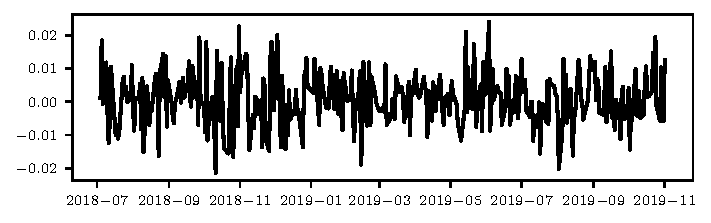
\includegraphics[width=\textwidth]{series.pdf}
	\caption{IMOEX Return}
	\label{fig:series}
\end{figure}

The data is reshaped to match usual input shape of Time Series DL models, which is a tensor [B, L, N], where B is batch size, L is sequence length and N is a number of variables. Therefore, one input of a model is a tensor of stacked matrices of the following form:

\begin{equation}
input = \begin{bmatrix} 
    y_{t} & x^{(1)}_{t} & \dots & x^{(n)}_{t} \\[1ex]
    y_{t-1} & x^{(1)}_{t-1} & \dots & x^{(n)}_{t-1} \\[1ex]
    y_{t-2} & x^{(1)}_{t-2} & \dots & x^{(n)}_{t-2} \\[1ex]
    \vdots & \vdots & \ddots & \vdots \\[1ex]
    y_{t-T} & x^{(1)}_{t-T} & \dots & x^{(n)}_{t-T} 
\end{bmatrix}
\end{equation}

The length of historic sequence considered at each step is a hyperparameter, and is chosen arbitrarily as 10, or 2 complete trading weeks.

Before feeding into a model, the data is normalized, i.e. each variable is demeaned and divided by its standard deviation. The scaling parameters are calculated only on training subset and applied to validation and test periods, to avoid information leakage.

Mean Squared Error is used as both Loss Function for training models and the main evaluation metric.

\begin{equation}
MSE = \frac{1}{N} \sum (y_t - \hat{y}_t)^2
\end{equation}

\begin{comment}
\begin{equation}
MDA = \frac{1}{N} \sum [ sign(\hat{y}_t)=sign(y_t) ]
\end{equation}

MSE directly measures squared deviation from the true value, making it the main metric for evaluating the performance of considered models. Directional accuracy is a simpler metric, evaluating only the correctness of predicted trend; it is used as an additional way to assess the quality of the models. Usage of this metric, should not be confused with classification problem, where only directions are forecasted in the first place, and models are specifically taught to predict classes via Cross Entropy loss functional.
\end{comment}

We employ Walk-Forward Cross Validation, a common validation scheme in time series forecasting, though underutilized in machine learning environment.
The data is sequentially split into 12 folds, one for each subsequent week of testing data. Each fold consists of 265 training instances, followed by validation and test periods, 5 days (a trading week) each. For each fold, the training period is used to train models, validation period is used to evaluate the set of hyperparameters and compare models of same architecture, and test period is used for final evaluation and comparison between different models.

\begin{figure}
	\centering
	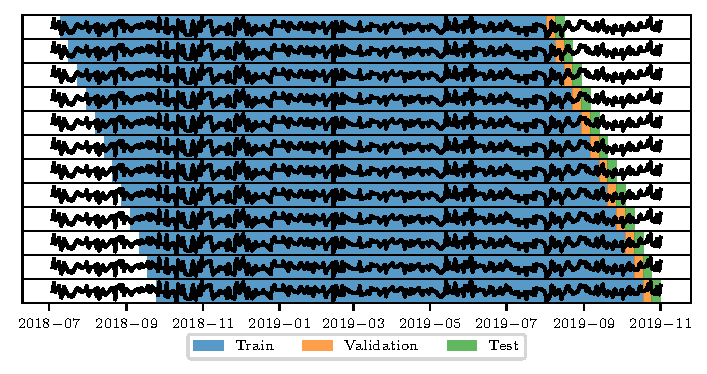
\includegraphics[width=\textwidth]{crossval.pdf}
	\caption{Walk-Forward Cross-Validation}
	\label{fig:walkforward}
\end{figure}

\begin{comment}
In contrast with dynamic or multiple-days-ahead forecasts, true values are input into the model for every subsequent day of the test period.
\end{comment}

We consider three model architectures and one naïve predictor:

\begin{itemize}

\item Naïve Zero

A baseline predictor, always predicting 0 as each day's return. Since all data is normalized, it corresponds to AR(0), estimated on training period.

\item LSTM

A vanilla LSTM model without any enhancements. Two hyperparameters are tuned for this model: number of layers (1, 2 or 4) and layer hidden size (16, 32 or 64). The final prediction is made by one fully-connected layer.

\begin{comment}
\item Bidirectional LSTM

LSTM Neural Network with twice the number of layers, iterating though input sequences in different directions. The hyperparameters are the same.
\end{comment}

\item CNN

Time series Convolutional Neural Network. Following X and Y, we construct it stacking 2 1D Convolution layers with ReLU activation functions, and Max Pooling layer, followed by another Convolution and Max Pooling pair. The hyperparameters for the model are filter sizes of Convolution layers (32-64-128, 64-128-256, 128-256-256, 256-512-1024), kernel sizes are fixed to 2.

\item CNN-LSTM

A hybrid architecture: CNN pre-processes inputs, extracting a new set of features, which are sequentially processed by LSTM. CNN part consists of 2 Convolution layers with ReLU activation functions, followed a Max Pooling layer. The hyperparameters are filter sizes (64-128, 128-256, 256-512, 512-1024), LSTM layers (1, 2, 4) and hidden size (16, 32 or 64).

\end{itemize}

All models are trained using Adaptive Momentum Stochastic Gradient Decent optimization algorithm (ADAM) with Learning Rate of 1e-3. All models are regularized by 10\% Dropout and 1e-3 Weight Decay.
Each of model specifications is trained 10 times, each time form a different weight initialization, to achieve better convergence. Best version of each model is chosen on each of validation periods.

After the models are trained, best sets of hyperparameters are selected for each of architectures based on validation metrics. To evaluate impacts of different variable groups on model performance, we exclude each of them, train the model again, and then compare the results.

Then, both global and local analysis of full models is performed using Gradient SHAP method \citep{lundberg_unified_2017}. SHAP explains each of model's outputs by providing a set of additive attributions for each of the model's input features. Summed together, they reconstruct model's output for this particular instance. Resulting attributions roughly represent how the model made its decision, making its insight human-readable and interpretable. In our 3-dimensional case, attribution for each test value follows input's shape, or the following form.

\begin{equation}
attributions = \begin{bmatrix} 
    \phi_{t} & \phi^{(1)}_{t} & \dots & \phi^{(n)}_{t} \\[1ex]
    \phi_{t-1} & \phi^{(1)}_{t-1} & \dots & \phi^{(n)}_{t-1} \\[1ex]
    \phi_{t-2} & \phi^{(1)}_{t-2} & \dots & \phi^{(n)}_{t-2} \\[1ex]
    \vdots & \vdots & \ddots & \vdots \\[1ex]
    \phi_{t-T} & \phi^{(1)}_{t-T} & \dots & \phi^{(n)}_{t-T} 
\end{bmatrix}
\end{equation}

\begin{equation}
\hat{y}_{t+1} = \sum_{v=0}^{n} \sum_{l=-T}^{0} \phi^{(v)}_l
\end{equation}

We aggregate absolute values of these attributions by different dimensions to get interpretations of relative importance across time lags, variables, variable groups, etc.

\section{Empirical Results}

\subsection{Model Performance}
\noindent

\begin{table}
\centering
\caption{\label{tab:res}Average Test MSE}
\begin{tabularx}{0.5\textwidth}{l|X}
Best Model               & MSE            \\ \hline
Naive Zero               & \textbf{0.8793} \\ \hline
CNN(128-256-512)         & \textbf{0.873}  \\
\textit{Sectors}         & 1.0061          \\
\textit{Shares}          & 0.951           \\
\textit{Currencies}      & 0.9916          \\
\textit{Commodities}     & 0.9182          \\
\textit{Foreign indexes} & 0.9642          \\
\textit{Bonds}           & 1.0135          \\ \hline
LSTM(16, 1)              & \textbf{1.0643} \\
\textit{Sectors}         & 1.3561          \\
\textit{Shares}          & 1.4998          \\
\textit{Currencies}      & 1.4968          \\
\textit{Commodities}     & 1.6165          \\
\textit{Foreign indexes} & 1.7486          \\
\textit{Bonds}           & 1.1959          \\ \hline
CNN-LSTM(256-512, 32, 2) & \textbf{0.8834} \\
\textit{Sectors}         & 0.9428          \\
\textit{Shares}          & 1.1223          \\
\textit{Currencies}      & 1.1447          \\
\textit{Commodities}     & 1.045           \\
\textit{Foreign indexes} & 0.9582          \\
\textit{Bonds}           & 1.0581
\end{tabularx}
\end{table}

\noindent Results of model evaluation are summarized in \autoref{tab:res}. As follows from comparison between the average MSE results and Zero Naïve predictor, we are unable to forecast Russian financial market any better than always predicting mean return over the previous year. Despite grid search over model hyperparameters, the best resulting models, CNN-LSTM(256-512, 32, 2) and CNN-LSTM(128-256-512) are only marginally close to the naïve case in terms of error. We can conclusively say, however, that this these architectures outperform basic LSTM. 
% Detailed results over 12 test weeks can be examined in Appendix.

\begin{figure}
	\centering
	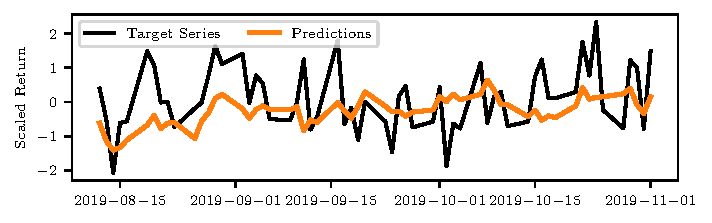
\includegraphics{preds.pdf}
	\caption{Best model predictions}
	\label{fig:preds}
\end{figure}

All models exhibit very unstable training, with validation outcome solely depending on weight initialization. For example, loss figures for period 1, for best CNN-LSTM model, look totally different under different initial states \autoref{fig:loss}. This can indicate that the performance issue may be not attributed to model design, but rather to training procedure: optimizer, starting from different initial states, arrives at totally different local minimas, all fitting the training data perfectly, yet unable to generalize to validation and test samples. We believe, however, that with sufficiently larger set of hyperparameters to try, specifically tinkering over the training procedure, and perhaps employing more data, stable results can be achieved in principle.

Analyzing the sets of used variables, we can conclude that, despite not being able to achieve results in general, the proposed macroeconomic features improve model performance. In \autoref{tab:res} italicized entries represent models trained on the set of features \textit{excluding} a particular group. Compared to the case with all variables included, reduced models all yield conclusively worse results.

\subsection{Feature attribution}

\noindent We proceed to explanation of model predictions using SHAP. For this section, only the best-performing CNN-LSTM model is considered.

As SHAP is able to explain each of predictions locally, this methodology is especially helpful for evaluating models in production. For instance, we can look at one of the days in the test period, 12-08-2019 (\autoref{fig:local}). This waterfall plot is interpreted as follows. The variables are sorted by their absolute Shapley values. At this specific day, all Gold variables were the most important in explaining model's prediction, pushing in into negatives; so did Novatek's variables, Euro exchange rates, MOEX sectoral index for finance, and others, with less absolute values. At the same time, changes in bond yields, index' past dynamics and a number of stocks drove expected value upwards.

By averaging absolute values of local attributions over all test instances, we  obtain global attributions, depicting relative importance of each feature for model's outputs across test period. As the input is a 3-dimensional tensor in our case, aggregations across different dimensions are analyzed.

\autoref{fig:lags} represents absolute values of Shapely explanations, averaged across all dimensions but the lag one. The graph shows that immediate lags are less important, than about 7-9 days into the past - this advocates for the existence of long-term tendencies, rather than short-term reactions to some news. The figure on the right shows that, attributions vary from day to day in the test sequence, and overall dynamic changes across time.

\begin{figure}
    \centering
    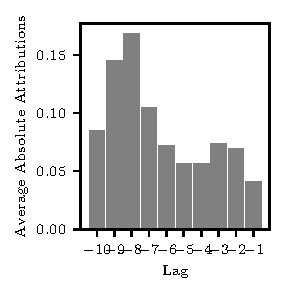
\includegraphics{lags.pdf}
    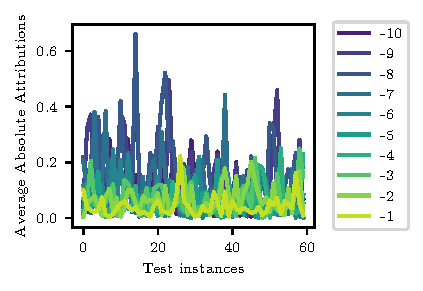
\includegraphics{lags_series.pdf}
    \caption{Lag importance}
    \label{fig:lags}
\end{figure}

\autoref{fig:vars_shap} presents SHAP variable attributions, averaged across Return-Volatility-HighLow-Volume sets for different instruments (detailed picture over all 101 features can be found in Appendix, \autoref{fig:all_vars_shap}). Interestingly enough, the first most important feature is Gold, and, in particular, its relative High-Low indicator. Generally, it does not contradict econometric empirical literature, as well as common sense; however, there are no studies on Russian stock market, which use Gold as explanatory variable, to support or oppose this result.

\begin{figure}
	\centering
	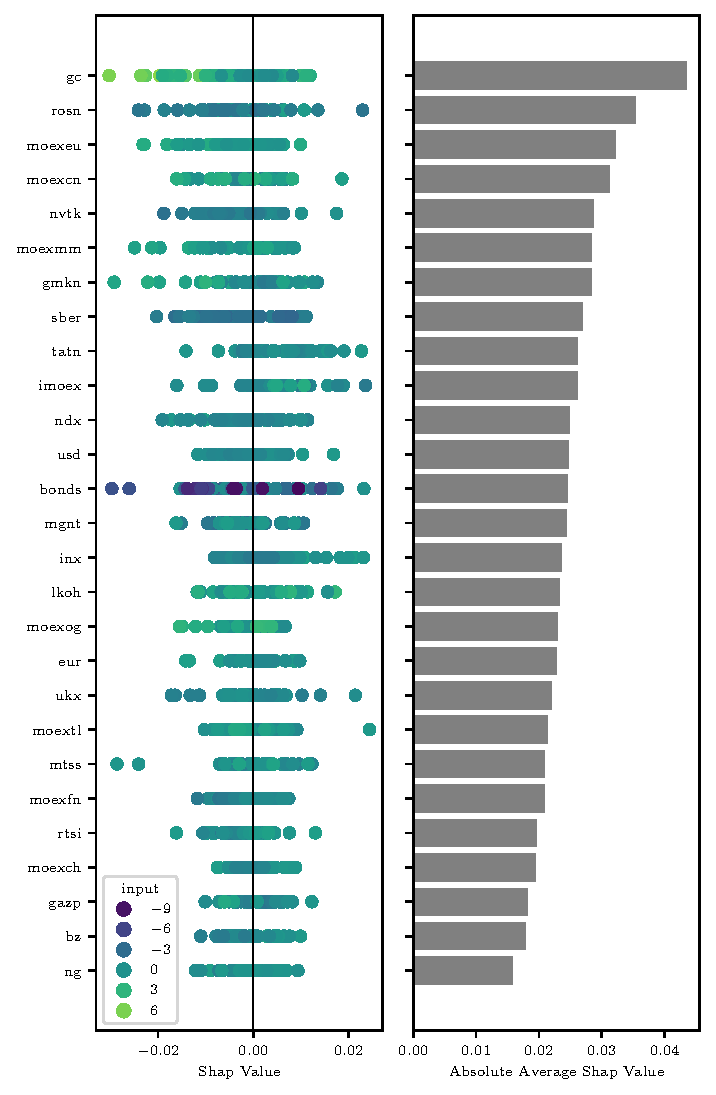
\includegraphics{beeswarm.pdf}
	\caption{Variable Attributions}
	\label{fig:vars_shap}
\end{figure}

Financial news of that period help reconstruct the story a bit better. 2019 was a splendid year for gold prices in general, and, in particular, so was September \citep{sieron_gold_2020, koh_gold_2019}. On September 3, Gold prices reached their (at that time) all-time peak of \$1546, having grown by 21.6\% in the last three months. Such rise is explained by several factors, including expectations of reduction in the U.S. federal funds rate and rising demand by Central Banks. Moreover, the time just before the global pandemic, Spring and Summer of 2019 were marked by pres. Trump's trade war with China, further increasing demand for hedging opportunities like Gold.

Our testing sample starts on Monday, 12th of August and ends on 1st of November, which corresponds exactly with that period. Therefore, the link between gold price and Russian stock market extracted by SHAP can be explained by Russian investors using gold as a hedge against increasing geopolitical risks; or, perhaps, gold fluctuations in this period just happened correlate with the general news sentiment. The presented feature attribution is by no means causal.

Another interesting observation is relative unimportance of the other considered commodities, Oil and Gas. Both of them ranked last among all other variables, despite both major Russian oil-producing companies' stocks ranking higher. While being somewhat surprising on the first glance, this result corresponds to empirical literature. Both works of \cite{korhonen_what_2016} and \cite{robert_d_gay_effect_2008} do not find oil prices driving Russian stock market as well for earlier periods, advocating for the argument for Russian economy being mature and diversified enough to not be affected by Oil prices.

Finally, it has to be noted, that those interpretations should be taken with a grain of salt. After all, as the forecasts themselves are not very accurate, so might be the attributions.

\begin{comment}
TODO:
finish LSTM and CNN models in intro
abstract
rewrite intro
add links to finam
\end{comment}

\section{Conclusion}

Deep learning methods are powerful ML methods applied in many prediction tasks, including one of financial time series forecasting.
Despite the predictive power of DL and its growing popularity, studies including fundamental macroeconomic factors are rarely conducted. While economists reserve to simpler linear methods, ML specialists tend to favor technical indicators above macroeconomic variables. We tried to integrate the two approaches. 

In this work we assess, whether including information on Exchange rates, Commodities, Sectors, Bonds Foreign markets and underlying Stocks can increase quality of predictions of IMOEX, a primary Russian stock market index. 
We considered three architectures: LSTM, CNN and CNN-LSTM. We did not come up with a sufficiently good forecasting model; best hyperparameter specifications ended up only marginally different from Zero Naive prediction in terms of MSE on test period, unable to forecast index returns reliably across different periods and different training runs. However, we still found out that including all of the considered variables is better for forecasts that leaving them out.

In addition to forecast quality analysis, we interpreted model predictions with a novel feature attribution method. We were able to extract a non-obvious relationship between IMOEX and gold prices in August-November of 2019, as well as other interpretable conclusions.

The main limitation, as well as a path for future research, is, of course, the models' predicting power. If the models can not forecast properly, then results regarding everything else have much less basis under them. 
However, we still have confidence in the fact that constructing and successfully training DL models is possible in proposed setup.

\bibliography{ref}
\clearpage

\section{Appendix}

\subsection{Used Packages \& Data}

\noindent All empirical work is done in Python \citep{van_rossum_python_2009}. Pandas and NumPy are used for data processing \citep{mckinney_data_2010,harris_array_2020}.
Neural networks are implemented in PyTorch \citep{paszke_pytorch_2019}. SHAP values are calculated with Captum \citep{kokhlikyan_captum_2020}. Figures are drawn by Matplotlib and Seaborn \citep{hunter_matplotlib_2007,waskom_seaborn_2021}.

All the data is openly available at finam.ru and investing.com \citep{noauthor_investingcom_nodate, noauthor_finam_nodate}. 

\subsection{Training procedure}

\begin{figure}[h]
	\centering
	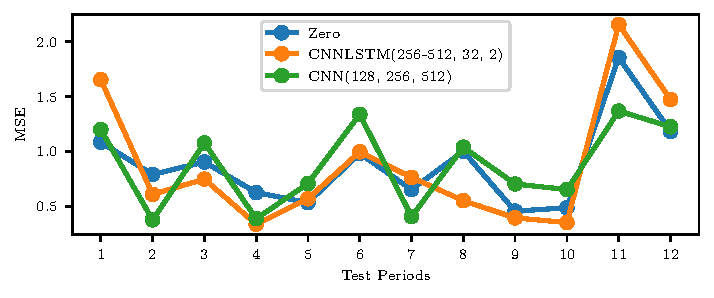
\includegraphics{periods.pdf}
	\caption{MSE on test periods}
	\label{fig:test_mse}
\end{figure}

\begin{figure}[h]
    \centering
    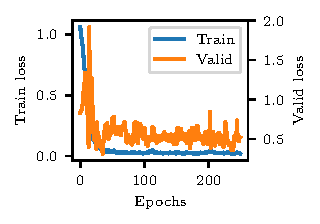
\includegraphics{good_loss.pdf}
    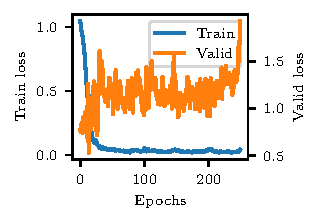
\includegraphics{bad_loss.pdf}
    \caption{Loss plots for 2 sets of initial weights}
    \label{fig:loss}
\end{figure}

\clearpage
\subsection{Data}

\begin{figure}[h]
	\centering
	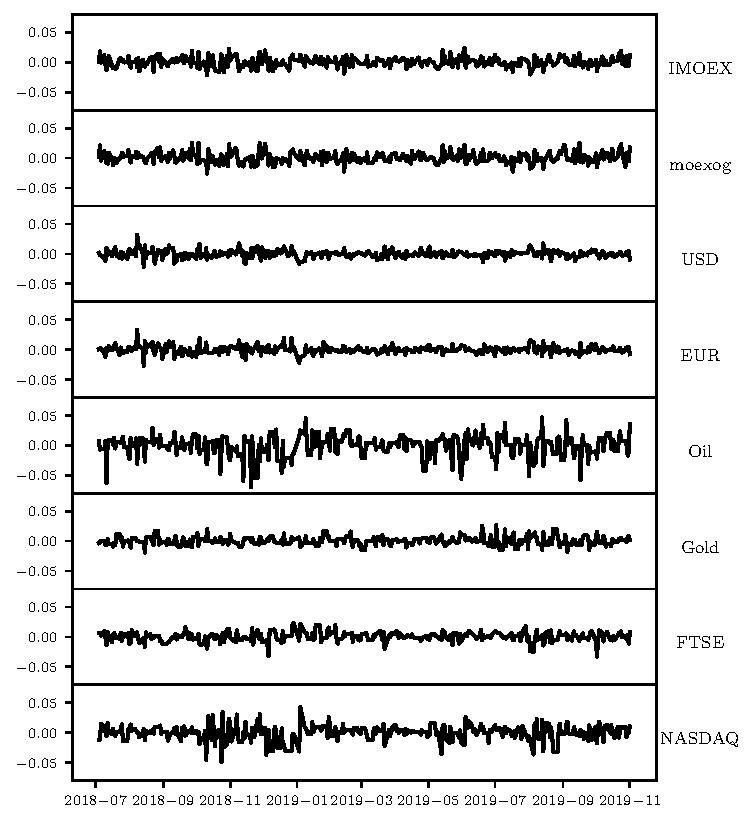
\includegraphics{data.pdf}
	\caption{Selected Returns across considered period}
	\label{fig:data}
\end{figure}

\clearpage
\subsection{SHAP values}

\begin{figure}[h]
    \centering
    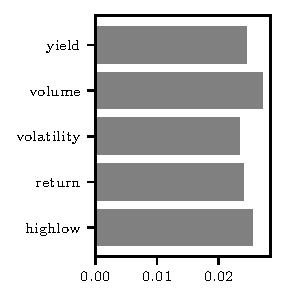
\includegraphics{types.pdf}
    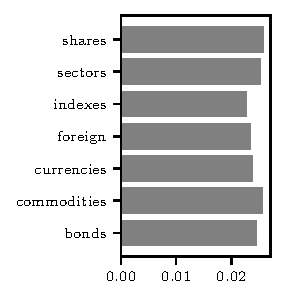
\includegraphics{classes.pdf}
    \caption{Average Abs SHAP values over variable types}
    \label{fig:types}
\end{figure}

\begin{figure}[h]
	\centering
	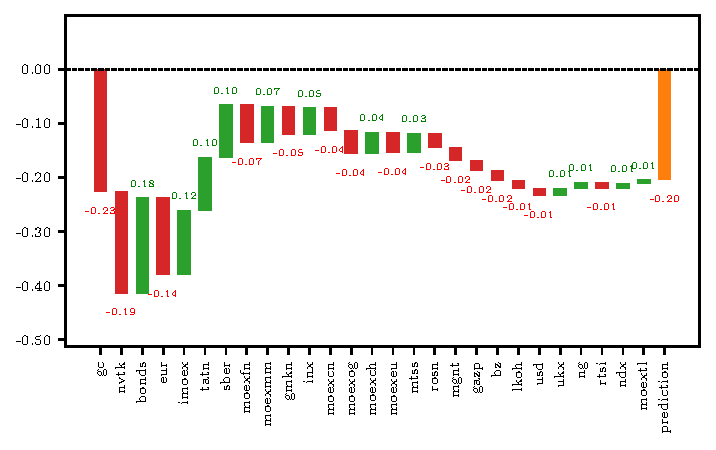
\includegraphics{local.pdf}
	\caption{Local explanations for 12-06-2019}
	\label{fig:local}
\end{figure}

\begin{figure}[h]
	\centering
	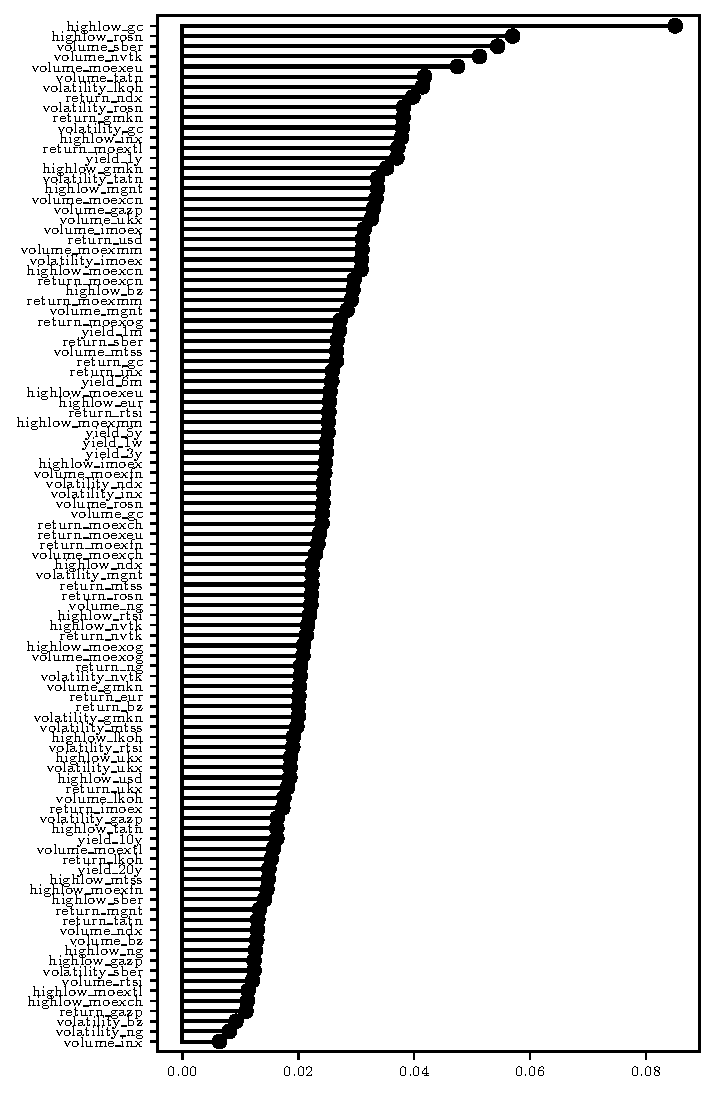
\includegraphics{all_vars_shap.pdf}
	\caption{Variable attributions}
	\label{fig:all_vars_shap}
\end{figure}

\end{document}
